%=====================================================================
%  CE-1115 Seguridad de la Informacion -- Proyecto, Parte 2
%  Informe de implementacion y despliegue
%  Cliente: Verdeazul Carbono S.A.
%  Tecnologico de Costa Rica -- Escuela de Ingenieria en Computadores
%  Prof. MSc. Andres Vargas Rivera -- Semestre II, 2026
%
%  Compilar dos veces:  pdflatex P2_Informe_grupo6.tex
%  La tabla del Anexo A sale de docs/cobertura.csv:  python generar_tabla.py
%=====================================================================
\documentclass[11pt,letterpaper]{article}

\usepackage[utf8]{inputenc}
\usepackage[T1]{fontenc}
\usepackage[spanish,es-noshorthands,es-tabla]{babel}
\usepackage{mathptmx}
\usepackage[defaultsans,scale=0.92]{lato}
\renewcommand{\ttdefault}{ptm}
\usepackage[letterpaper,margin=2.4cm,headheight=15pt]{geometry}
\usepackage{microtype}
\usepackage{amsmath,amssymb}
\usepackage{xcolor}
\usepackage{colortbl}
\usepackage{booktabs,tabularx,array,longtable,multirow}
\usepackage{enumitem}
\usepackage{titlesec}
\usepackage{fancyhdr}
\usepackage[most]{tcolorbox}
\usepackage{tikz}
\usetikzlibrary{positioning,arrows.meta,calc,fit}
\usepackage{caption}
\usepackage{float}
\usepackage{graphicx}
\usepackage{needspace}
\usepackage{fancyvrb}
\usepackage{fvextra}
\usepackage[hidelinks]{hyperref}

%--------------------------- datos del grupo -------------------------
\newcommand{\numgrupo}{6}
\newcommand{\titulodoc}{Informe de implementación y despliegue}
\newcommand{\subtitulodoc}{Verdeazul Carbono en Cloud Run, Neon y Secret Manager}
\newcommand{\titulocorto}{Implementación y despliegue}
\newcommand{\fechaentrega}{19 de noviembre de 2026}

%--------------------------- estilo ----------------------------------
% Todo el texto va en negro; los diagramas usan grises.
\definecolor{tinta}{HTML}{1A1A1A}
\definecolor{gris}{HTML}{5F5E5A}
\definecolor{regla}{HTML}{B9B8B0}
\definecolor{fondo}{HTML}{F2F1EC}

\titleformat{\section}{\Large\rmfamily\bfseries }{\thesection}{0.6em}{}
\titleformat{\subsection}{\large\rmfamily\bfseries }{\thesubsection}{0.6em}{}
\titlespacing*{\section}{0pt}{1.2em}{0.4em}
\titlespacing*{\subsection}{0pt}{0.8em}{0.25em}
\setlength{\parindent}{0pt}
\setlength{\parskip}{0.5em}
\setlist{leftmargin=1.5em,itemsep=2pt,topsep=3pt,parsep=0pt}
\captionsetup{font=small,labelfont=bf,skip=5pt}

\pagestyle{fancy}
\fancyhf{}
\fancyhead[L]{\small\rmfamily CE-1115 $\cdot$ Proyecto Parte 2 $\cdot$ Grupo \numgrupo}
\fancyhead[R]{\small\rmfamily \titulocorto}
\fancyfoot[C]{\small\rmfamily \thepage}
\renewcommand{\headrulewidth}{0.4pt}

\newcolumntype{L}[1]{>{\raggedright\arraybackslash}p{#1}}
\newcolumntype{Y}{>{\raggedright\arraybackslash}X}
\newcommand{\cab}[1]{\textbf{\rmfamily #1}}
\newcommand{\cod}[1]{\texttt{\small #1}}
\newcommand{\arch}[1]{\texttt{\small #1}}
\newtcolorbox{nota}{enhanced,breakable,colback=white,colframe=black,
  boxrule=0pt,leftrule=3pt,arc=0pt,left=8pt,right=8pt,top=5pt,bottom=5pt}
\newtcolorbox{salida}{enhanced,breakable,colback=fondo,colframe=fondo,
  boxrule=0pt,arc=0pt,left=6pt,right=6pt,top=4pt,bottom=4pt}
\fvset{fontsize=\scriptsize,breaklines=true,breakanywhere=true}

\begin{document}

%=====================================================================
%  PORTADA
%=====================================================================
\begin{titlepage}
\centering
\vspace*{0.6cm}
{\large\scshape Instituto Tecnológico de Costa Rica}\\[0.2cm]
{\large\scshape Escuela de Ingeniería en Computadores}\\[0.2cm]
{\large CE-1115 Seguridad de la Información}\\[1.5cm]

{\rule{\textwidth}{1.4pt}}\\[0.6cm]
{\rmfamily\large Proyecto $\cdot$ Parte 2 $\cdot$ Implementación y despliegue seguro}\\[0.45cm]
{\rmfamily\bfseries\fontsize{24}{29}\selectfont \titulodoc}\\[0.35cm]
{\rmfamily\large \subtitulodoc}\\[0.6cm]
{\rule{\textwidth}{1.4pt}}\\[1.1cm]

{\large\bfseries Cliente}\\[0.25cm]
{\large Verdeazul Carbono S.A.}\\[0.1cm]
{Certificación de captura de carbono $\cdot$ Pérez Zeledón, Costa Rica}\\[1.1cm]

{\large\bfseries Grupo \numgrupo}\\[0.4cm]
\begin{tabular}{@{}l@{\hspace{1.4cm}}l@{}}
\toprule
\textbf{Integrante} & \textbf{Carné} \\
\midrule
Randall Bryan Bolaños López & 2019043784 \\
Javier Tenorio Cervantes    & 2020065308 \\
Julio Varela Venegas        & 2019008041 \\
Axel Flores Lara            & 2021453573 \\
\bottomrule
\end{tabular}\\[1.1cm]

{\large Prof. MSc. Andrés Vargas Rivera}\\[0.15cm]
{\large Semestre II, 2026}

\vfill
{\large\bfseries Fecha de entrega: \fechaentrega}
\end{titlepage}

\pagenumbering{roman}
\tableofcontents
\newpage
\pagenumbering{arabic}

%=====================================================================
\section{Qué quedó en línea}
%=====================================================================

El sistema que diseñamos en la Parte 1 corre en Google Cloud Run con la base en Neon. Cualquiera lo
abre desde internet por HTTPS:

\begin{center}
\small
\begin{tabularx}{\textwidth}{@{}L{4.2cm} Y@{}}
\toprule
\cab{Qué} & \cab{Dónde} \\
\midrule
Aplicación (siete roles) & \url{https://verdeazul-app-708901712393.us-east1.run.app} \\
Comprobación pública de certificados & \url{https://verdeazul-publico-708901712393.us-east1.run.app} \\
Repositorio (público) & \url{https://github.com/Randall-BL/ProyectoSeguridad} \\
Versión desplegada & \cod{v1.0.1}: las cinco imágenes y la etiqueta de git salen del mismo commit \\
Credenciales de prueba & Anexo para el profesor, entregado aparte (nunca en el repositorio) \\
\bottomrule
\end{tabularx}
\end{center}

Implementamos la matriz completa de la Parte 1: los 102 permisos concedidos de los diez roles y las 38
celdas denegadas, con las reglas C1 a C20 y los controles de historial H1 a H4. Construimos en cuatro
sprints, cada uno desplegado en la nube antes de seguir (\cod{v0.1.0} el 6 de noviembre, solo
«hola»; \cod{v0.2.0} a \cod{v0.4.0}; \cod{v1.0.0} y \cod{v1.0.1} el 15). El \cod{README} explica cómo desplegar y
lista cada versión publicada.

%=====================================================================
\section{Arquitectura desplegada}
%=====================================================================

La figura~\ref{fig:arquitectura} muestra lo que de verdad corre. Cada componente de la Parte 1 existe
como pieza propia, con su imagen, su cuenta de servicio y su usuario de base. Las fronteras F1 a F5
son las del documento de arquitectura.

\begin{figure}[H]
\centering
\begin{tikzpicture}[
  font=\scriptsize,
  caja/.style={draw=black,thick,rounded corners=2pt,align=center,inner sep=3pt,text width=#1,fill=white},
  caja/.default=2.9cm,
  ext/.style={draw=black,dashed,rounded corners=2pt,align=center,inner sep=3pt,text width=1.8cm},
  flecha/.style={-{Stealth[length=1.8mm]},thick},
  fr/.style={font=\scriptsize\bfseries,fill=white,inner sep=1pt}]
  % fila de arriba: de dónde llegan la imagen, la política y los secretos
  \node[caja=2.4cm] (ar)  at (3.0,3.0) {Artifact Registry\\5 imágenes \texttt{v1.0.1}};
  \node[caja=2.6cm] (opa) at (6.6,3.0) {\textbf{politica} (OPA)\\solo \texttt{localhost:8181}};
  \node[caja=2.6cm] (sm)  at (10.6,3.0) {\textbf{Secret Manager}\\un lector por secreto};
  % servicios
  \node[ext] (nav)  at (0,1.0)  {Navegador\\(siete roles)};
  \node[ext] (comp) at (0,-2.2) {Comprador\\(rol PUB)};
  \node[caja=2.2cm] (gfe) at (3.0,-0.6) {Frente de Google\\TLS; HTTP a HTTPS};
  \node[caja] (app) at (6.6,1.0) {\textbf{verdeazul-app}\\Django, punto de cumplimiento\\\texttt{sa-app} $\cdot$ \texttt{va\_app}};
  \node[caja=2.6cm] (pub) at (5.8,-2.2) {\textbf{verdeazul-publico}\\\texttt{sa-publico} $\cdot$ \texttt{va\_publico}};
  \node[caja=2.7cm] (emi) at (10.6,1.0) {\textbf{verdeazul-emision}\\privado $\cdot$ \texttt{sa-emision}\\\texttt{va\_emision}};
  \node[caja=2.5cm] (job) at (14.3,-0.9) {\textbf{verdeazul-trabajos}\\Job diario $\cdot$ \texttt{sa-trabajos}\\\texttt{va\_trabajos}};
  \node[ext,text width=1.6cm] (sch) at (14.3,1.0) {Cloud\\Scheduler};
  \node[ext,text width=1.6cm] (tsa) at (14.3,-3.3) {TSA pública\\RFC 3161};
  \node[caja=4.4cm] (neon) at (10.6,-3.6) {\textbf{Neon}: PostgreSQL 18 + PostGIS\\seguridad por fila, disparadores\\y bitácora encadenada};

  \draw[flecha] (nav) -- node[fr,above,sloped]{F1} (gfe);
  \draw[flecha] (comp) -- node[fr,below,sloped]{F1} (gfe);
  \draw[flecha] (gfe) -- node[fr,above,sloped]{F2} (app);
  \draw[flecha] (gfe) -- node[fr,below,sloped]{F2} (pub);
  \draw[flecha] (app) -- node[fr,right]{F3} (opa);
  \draw[flecha] (app) -- node[above,font=\scriptsize,align=center]{token\\IAM} (emi);
  \draw[flecha] ([xshift=-0.25cm]app.south east) -- ([xshift=-0.25cm]app.south east |- neon.west) -- node[fr,above]{F4} (neon.west);
  \draw[flecha] (pub.south) |- node[fr,pos=0.75,below]{F4} ([yshift=-0.35cm]neon.west);
  \draw[flecha] (emi) -- node[fr,right]{F4} (neon);
  \draw[flecha] (job) -- node[fr,above,sloped]{F4} (neon.north east);
  \draw[flecha] (job.north west) -- node[above,sloped,font=\scriptsize]{pendientes} (emi.south east);
  \draw[flecha] (sch) -- (job);
  \draw[flecha] (job) -- node[fr,right]{F5} (tsa);
  \draw[flecha,dashed] (sm) -- (emi);
  \draw[flecha,dashed] (ar) -| (app.north west);
\end{tikzpicture}
\caption{Arquitectura desplegada, con las fronteras F1 a F5 de la Parte 1. Las flechas continuas son
peticiones; las punteadas, de dónde llegan la imagen y los secretos (cada servicio lee solo los suyos;
se dibuja el de la clave de firma). El verificador de consola (\arch{verificador/}) no aparece porque
corre sin conexión, en la máquina de quien compra.}
\label{fig:arquitectura}
\end{figure}

\begin{center}
\footnotesize
\renewcommand{\arraystretch}{1.12}
\begin{tabularx}{\textwidth}{@{}L{2.5cm} L{2.6cm} L{2.4cm} Y@{}}
\toprule
\cab{Componente (Parte 1)} & \cab{En Cloud Run} & \cab{Usuario de base} & \cab{Qué puede} \\
\midrule
Aplicación y punto de cumplimiento & servicio \cod{verdeazul-app} & \cod{va\_app} & Leer y escribir el negocio, filtrado por la seguridad por fila; nunca borrar; solo leer certificados. \\
Motor de decisión & contenedor \cod{politica} en la misma instancia & — & Decidir cada petición. No tiene puerto expuesto: solo lo alcanza la aplicación. \\
Emisión (fila SIS) & servicio privado \cod{verdeazul-emision} & \cod{va\_emision} & Leer lo necesario e insertar certificados; revocar es solo \cod{UPDATE} de estado. Único lector de la clave de firma. \\
Comprobación pública (fila PUB) & servicio \cod{verdeazul-publico} & \cod{va\_publico} & Nada sobre tablas: solo llamar a \cod{va\_comprobar(código)}. \\
Trabajos programados & Cloud Run Job \cod{verdeazul-trabajos} & \cod{va\_trabajos} & Vencer asignaciones y cuentas, cerrar sesiones, escalar alertas, verificar la cadena y guardar el testigo. \\
\bottomrule
\end{tabularx}
\end{center}

Cada imagen se construye con Cloud Build desde un commit que ya está en GitHub, y se publica con dos
etiquetas, la versión y \cod{git-<commit>}; nunca \cod{latest}. Todas corren con un usuario sin
privilegios (\cod{USER 10001}; OPA, \cod{1000}), con la base de Python fijada por huella, dependencias
con versión y huella (\cod{pip install --require-hashes}) y sin \cod{pip} dentro de la imagen final.

%=====================================================================
\section{Controles implementados}
%=====================================================================

Para cada control obligatorio indicamos dónde está en el código y cómo comprobamos que funciona.
Todas las pruebas corren en el CI de GitHub en cada cambio (sección~\ref{sec:pruebas}).

\begin{center}
\footnotesize
\renewcommand{\arraystretch}{1.15}
\begin{tabularx}{\textwidth}{@{}L{2.6cm} Y Y@{}}
\toprule
\cab{Control} & \cab{Dónde} & \cab{Cómo se verifica} \\
\midrule
1. Contraseñas con hash lento &
Argon2id con sal por usuario: \arch{app/verdeazul/settings.py:128}. Política de longitud y de
contraseñas comunes en los validadores. &
\cod{cuentas.tests.HashDeContrasenas}: el valor guardado empieza con \cod{argon2\$argon2id\$} y dos
cuentas con la misma contraseña no tienen el mismo hash. En Neon, ninguna fila tiene otro algoritmo. \\
\midrule
2. Control de acceso del lado del servidor &
Cada ruta lleva \cod{@protegida(verbo, objeto)} (\arch{app/autorizacion/proteccion.py:57}), que
pregunta al motor OPA con hechos tomados de la base, nunca de la petición
(\arch{app/autorizacion/motor.py:66}). Si el motor no responde, se deniega (K-3). Segundo candado en
la base: seguridad por fila (\arch{app/negocio/sql/0003}), disparadores
(\arch{app/negocio/sql/0004}, \arch{0006}, \arch{0007}) y permisos por usuario de base
(\arch{app/negocio/sql/0002}). &
Los 41 casos de la Parte 1 por las rutas; el caso feliz de los 102 permisos; 174 intentos con
identificadores ajenos con cada rol, como \cod{va\_app}; cada regla repetida en OPA y en la base
(\cod{flujos.tests\_equivalencia}); 71 pruebas de Rego. \\
\midrule
3. Secretos fuera del código &
Los siete secretos viven en Secret Manager (sección~\ref{sec:secretos}). El código los lee del
entorno (\arch{app/verdeazul/settings.py}); los YAML de Cloud Run los inyectan con versión fija. &
gitleaks sobre los 98 commits de la historia en el CI y en un gancho local; \cod{.gitignore} rechaza
\cod{.env}, llaves y archivos de cuentas de prueba. \\
\midrule
4. TLS en todo el tráfico &
Cloud Run solo expone HTTPS. Django redirige y manda HSTS de un año
(\arch{app/verdeazul/settings.py:223--225}). Hacia Neon: \cod{sslmode=verify-full} y
\cod{channel\_binding=require} en cada cadena de conexión. &
Evidencia de la sección~\ref{sec:evidencia}: HTTP responde 302 hacia HTTPS con HSTS. Mozilla HTTP
Observatory y ZAP sobre la URL pública (sección~\ref{sec:escaneos}). \\
\midrule
5. Validación de entradas &
Formularios de Django con tipo y rango en cada campo; todo acceso a datos por el ORM o
\cod{cursor.execute(sql, parámetros)}, sin \cod{raw()} ni \cod{extra()}. El servicio público valida
el formato del código antes de ir a la base y limita el tamaño de lo que se sube. &
Ruff con las reglas de seguridad (S608) y bandit (B608) en el CI; las pruebas de IDOR y de C2 envían
valores fuera de rango; ZAP en modo base sin alertas de inyección. \\
\midrule
6. Firma digital de los certificados &
Ed25519 sobre JSON canónico, con la clave pública y su huella incrustadas
(\arch{verificador/verdeazul\_certificado.py:65}). Firma solo el servicio de emisión
(\arch{emision/emitir.py:110}), único lector de la clave. La verificación exige además que la clave
incrustada sea la publicada (\arch{verdeazul\_certificado.py:118}). &
Un certificado válido pasa; el mismo con una tonelada cambiada falla; uno firmado con otra clave se
rechaza; en el servicio público y en el verificador sin conexión (\cod{docs/demostracion/}). \\
\bottomrule
\end{tabularx}
\end{center}

\begin{nota}
\textbf{Lo que el servidor decide, aunque la interfaz no lo muestre.} La interfaz solo enseña las
acciones que la celda del rol permite, pero eso es comodidad: la prueba \cod{flujos.tests\_idor}
envía, con cada rol, cada petición directamente, sin pasar por los botones, y ninguna se ejecuta
fuera de lo permitido. Además, para un técnico o un dueño, un identificador ajeno responde igual que
uno inexistente (404), así que la respuesta no revela qué existe.
\end{nota}

%=====================================================================
\section{Gestión de secretos}\label{sec:secretos}
%=====================================================================

\begin{center}
\footnotesize
\renewcommand{\arraystretch}{1.12}
\begin{tabularx}{\textwidth}{@{}L{3.2cm} L{2.2cm} Y L{1.2cm}@{}}
\toprule
\cab{Secreto} & \cab{Único lector} & \cab{Cómo llega} & \cab{Versión} \\
\midrule
\cod{django-secret-key} & \cod{sa-app} & Variable \cod{DJANGO\_SECRET\_KEY} & 1 \\
\cod{mfa-clave} & \cod{sa-app} & \cod{MFA\_CLAVE}: cifra con Fernet los secretos TOTP en la base & 1 \\
\cod{db-url-app} & \cod{sa-app} & \cod{DATABASE\_URL} del usuario \cod{va\_app} & 1 \\
\cod{db-url-emision} & \cod{sa-emision} & \cod{DATABASE\_URL} de \cod{va\_emision} & 1 \\
\cod{db-url-publico} & \cod{sa-publico} & \cod{DATABASE\_URL} de \cod{va\_publico} & 1 \\
\cod{db-url-trabajos} & \cod{sa-trabajos} & \cod{DATABASE\_URL} de \cod{va\_trabajos} & 1 \\
\cod{firma-clave-privada} & \cod{sa-emision} & \cod{FIRMA\_CLAVE}: los 32 bytes de la semilla Ed25519 & 1 \\
\bottomrule
\end{tabularx}
\end{center}

\begin{itemize}
  \item \textbf{Dónde viven.} En Secret Manager, replicados solo en \cod{us-east1}. Cada uno con un
    único lector, la cuenta de servicio del componente que lo usa, dado sobre el secreto y no sobre el
    proyecto. Nadie del equipo puede actuar como ninguna cuenta de servicio (\cod{docs/iam.md}).
  \item \textbf{Cómo llegan.} Cloud Run los inyecta como variables de entorno con
    \cod{secretKeyRef} y una versión fija: rotar un secreto es un cambio visible en el YAML del
    servicio. No aparecen en ningún \cod{Dockerfile} ni en la imagen.
  \item \textbf{Cómo se crearon.} \arch{infra/crear-secretos.sh} genera cada valor y lo manda a
    Secret Manager por la entrada estándar: nunca pasa por un archivo ni por la pantalla. La clave
    de firma se genera en Python, la pública se escribe en \cod{docs/} y la privada viaja por una
    tubería a \cod{gcloud}; el mismo script comprueba después que ambas corresponden.
  \item \textbf{Lo que no es un secreto.} La clave pública de Verdeazul está en el README, en
    \cod{docs/verdeazul-clave-publica.pem} y en \cod{/.well-known/verdeazul-clave.pem} del servicio
    público. Huella SHA-256: \cod{5fb2e24f\ldots166d0f}.
  \item \textbf{Cuentas de prueba.} Contraseñas y semillas TOTP de los doce personajes van en el
    anexo para el profesor, fuera del repositorio.
\end{itemize}

%=====================================================================
\section{Seguridad heredada de la plataforma}
%=====================================================================

\subsection{Neon}

\textbf{Lo que protege sin que hagamos nada.} Cifra los datos en reposo y exige TLS en toda conexión.
Aísla cada proyecto en su propio cómputo. Guarda el historial para recuperar la base a un punto en
el tiempo dentro de la ventana del plan. Autentica cada conexión con usuario y contraseña (SCRAM).

\textbf{Lo que configuramos y por qué.}
\begin{itemize}
  \item \textbf{Conexión.} Por el agrupador de conexiones (\emph{pooler}), con \cod{verify-full}
    contra las autoridades de la imagen y \cod{channel\_binding=require}, que impide que un
    intermediario reenvíe la autenticación. Descartamos \cod{sslmode=require}, que cifra pero no
    comprueba con quién habla.
  \item \textbf{Usuarios.} Un usuario por componente, ninguno dueño de tablas ni con atributos de
    administración (lo comprueba \arch{db/roles/servicio.sql}). La aplicación no puede borrar en
    ninguna tabla del negocio. El dueño solo se usa para migrar, desde la máquina del equipo.
  \item \textbf{El segundo candado en la base.} Seguridad por fila para C1 y C5, disparadores para
    C2, C3, C4, C8, C10, C11, C14, C16 y C19, y una bitácora encadenada en la que nadie, ni el dueño,
    modifica ni borra.
  \item \textbf{Ramas.} \cod{main} para el despliegue y \cod{dev} para probar migraciones. Las pruebas
    automáticas corren en una base local o en la del CI, nunca contra Neon.
  \item \textbf{Direcciones de origen.} No restringimos IP. Cloud Run sale por direcciones que no
    son fijas, y fijarlas exige un conector con NAT (de pago) más un plan de Neon que permita listas
    de IP. La compensación es que cada credencial solo abre su usuario mínimo.
\end{itemize}

\textbf{Lo que sigue siendo nuestro.} Neon no protege contra una consulta mal construida (por eso
consultas parametrizadas y ruff/bandit en el CI), contra un permiso excesivo (cuatro usuarios
mínimos, probados en \cod{flujos.tests\_equivalencia}) ni contra una credencial filtrada (secretos con
un único lector y gitleaks). Tampoco cubre a quien tiene la credencial del dueño: puede desactivar un
disparador y alterar la bitácora. La cadena de huellas lo delata y el trabajo diario guarda un sello
de tiempo RFC 3161 de una autoridad externa, que prueba que esa huella ya existía (amenaza de la
Parte 1 contra la integridad del registro).

\subsection{Cloud Run}

Google protege la infraestructura y aísla cada instancia en su propio entorno de ejecución (gVisor o
una microVM, según la generación). Termina el TLS con certificados
que renueva solo, y comprueba el token de identidad antes de dejar pasar una petición a un servicio
privado. Nosotros respondemos por lo que hay dentro:
\begin{itemize}
  \item el código y sus dependencias: Trivy, pip-audit y Dependabot;
  \item quién puede invocar qué: solo \cod{sa-app} y \cod{sa-trabajos} llegan a la emisión, y el
    servicio vuelve a revisar la cuenta del token;
  \item los secretos y la cuenta con la que corre cada servicio, que nunca es la de Compute;
  \item las cabeceras de la aplicación: CSP sin scripts, HSTS, COOP, CORP y COEP.
\end{itemize}

%=====================================================================
\section{Desviaciones respecto al diseño}
%=====================================================================

\begin{center}
\footnotesize
\renewcommand{\arraystretch}{1.12}
\begin{longtable}{@{}L{0.8cm} L{4.2cm} L{4.6cm} p{5.0cm}@{}}
\toprule
\cab{N.º} & \cab{Qué cambió} & \cab{Por qué} & \cab{Implicación de seguridad} \\
\midrule
\endhead
D-01 & Sin el proxy Caddy: TLS y HSTS los dan el frente de Google y Django; el tamaño, Django. & Cloud Run ya termina TLS y solo expone HTTPS. & La frontera F1 la valida Google y no un componente nuestro. El límite de ritmo quedó en el inicio de sesión (esperas crecientes y bloqueo) y en la comprobación pública, no en cada ruta. \\
D-02 & Neon en lugar de PostgreSQL propio. & Lo fija el enunciado. & El superusuario real es del proveedor; ganamos cifrado en reposo y recuperación a un punto en el tiempo. \\
D-03 & Secret Manager en lugar de la bóveda OpenBao. & Lo fija el enunciado. & El servicio de emisión lee la clave (la bóveda firmaba sin entregarla). Se acota con un único lector. La alternativa, Cloud KMS, firma sin entregar la clave pero tiene costo. \\
D-04 & Respaldos de Neon. & Vienen con la plataforma. & Se pierde el respaldo cifrado en otro proveedor con llave propia. \\
D-05 & Cloud Run en lugar de un servidor con Podman. & Lo fija el enunciado. & Se pierde SELinux y se gana el aislamiento de Cloud Run entre instancias; el contenedor sigue sin root. \\
D-06 & Máximo de 20 asignaciones activas por técnico (K-1). & Acotar cuánto alcanza una cuenta. & Un técnico comprometido llega a 20 fincas, no al catálogo. Es un parámetro que aprueba GER. \\
D-07 & Segundo factor TOTP para todos, sin llaves de acceso. & Las cuentas de prueba se usan desde cualquier equipo. & Un código temporal puede pedirse en una página falsa; la llave de acceso lo evitaría. Nadie puede quitarse el segundo factor. \\
D-08 & Testigo externo: sello RFC 3161 diario de una TSA pública (DigiCert o FreeTSA), sin buzón del auditor. & Lo mínimo defendible sin costo. & Detecta que alguien con acceso a la base quite registros recientes; no detecta lo hecho en el mismo día antes del sello. \\
D-09 & La comprobación pública usa una función (\cod{va\_comprobar}) en lugar de una vista. & Código exacto y sin búsquedas por construcción. & Más estricto que el diseño: \cod{va\_publico} no lee ninguna tabla. El límite de ritmo vive en la memoria de la única instancia. \\
D-10 & Los trabajos programados también invocan la emisión. & Recuperar una emisión que falló después de aprobar. & Una cuenta más llega al servicio privado; solo puede pedir lo pendiente, y la base vuelve a exigir C4. \\
D-11 & El certificado es un JSON firmado; no hay versión en PDF con QR. & El tiempo se fue a la matriz y a los controles. & La verificación no cambia; la versión legible la da el servicio público. \\
\bottomrule
\end{longtable}
\end{center}

%=====================================================================
\section{Cobertura de la matriz}
%=====================================================================

La tabla completa, permiso por permiso, está en el Anexo~A y en \cod{docs/cobertura.md}. La genera
\arch{infra/cobertura.py} a partir de \cod{matriz.json}, del código (regla de Rego, ruta, candado de
la base) y del registro de una corrida de las pruebas, así que no se edita a mano. Resumen por regla:

\begin{center}
\scriptsize
\renewcommand{\arraystretch}{1.0}
\begin{longtable}{@{}p{1.0cm} p{4.6cm} p{2.4cm} p{2.7cm} p{2.9cm} p{1.2cm}@{}}
\toprule
\cab{Regla} & \cab{Nombre} & \cab{Motor} & \cab{Base} & \cab{Casos T} & \cab{Pruebas} \\
\midrule
\endhead
C1 & Asignación vigente & reglas.rego:17 & negocio 0003, negocio 0005, negocio 0007 & T-01, T-02, T-27 & 6  \\
C2 & Edición solo en borrador & reglas.rego:34 & negocio 0004 & T-01, T-03, T-04, T-21, T-30 & 11  \\
C3 & Quien registró no aprueba (K-2) & reglas.rego:51 & negocio 0004 & T-05, T-06, T-17, T-26, T-40 & 10  \\
C4 & Emisión única & reglas.rego:58 & negocio 0002, negocio 0006 & T-07, T-25 & 5  \\
C5 & Solo lo suyo & reglas.rego:72 & negocio 0003, negocio 0007 & T-08 & 3  \\
C6 & Ventana de auditoría & reglas.rego:84 & — & T-09 & 3  \\
C7 & Solicitar enmienda & reglas.rego:88 & — & T-11, T-21 & 4  \\
C8 & Autorización final & reglas.rego:95 & negocio 0004 & T-12, T-24 & 4  \\
C9 & Corregir dentro del plazo & reglas.rego:105 & — & T-13 & 2  \\
C10 & Revisión técnica independiente & reglas.rego:113 & negocio 0004 & T-14, T-23 & 4  \\
C11 & Catálogo con segunda firma & reglas.rego:122 & negocio 0004 & T-15 & 1  \\
C12 & Nadie se administra a sí mismo & reglas.rego:132 & negocio 0004 & T-16 & 2  \\
C13 & Credenciales y declaración propias & reglas.rego:145 & — & T-35 & 2  \\
C14 & Apertura y cierre entre dos & reglas.rego:149 & negocio 0004 & T-04, T-17, T-22 & 6  \\
C15 & Alertas ajenas & reglas.rego:164 & negocio 0006 & T-36 & 2  \\
C16 & Supresión condicionada & reglas.rego:177 & negocio 0004 & T-37 & 2  \\
C17 & Abstención por vínculo & decision.rego:80 & — & T-29 & 2  \\
C18 & Exportar evidencia & reglas.rego:180 & — & T-31 & 3  \\
C19 & Asignar con vigencia y máximo de activas (K-1) & reglas.rego:185 & negocio 0004, negocio 0007 & T-27, T-28, T-38, T-39 & 8  \\
C20 & Comprobación pública & reglas.rego:193 & negocio 0006 & T-32 & 4  \\
H1 & Frecuencia & decision.rego:55 & — & T-02, T-18 & 4  \\
H2 & Tiempo & decision.rego:108 & — & T-34 & 2  \\
H3 & Combinada & decision.rego:105 & — & T-19, T-33 & 4  \\
H4 & Secuencia (C3, C8, C10) & reglas.rego:51 & negocio 0004 & T-06, T-14, T-24 & 6  \\
K-3 & Motor caído: fallo cerrado & decision.rego:39 & — & T-41 & 4  \\
Filas & Filas sin acceso (AUD no escribe, OPE no entra) & — & — & T-10, T-20 & 3  \\
\bottomrule
\end{longtable}
\end{center}


Los 102 permisos tienen su prueba en verde: los 68 que se ejercen desde una pantalla, con una prueba
generada desde la matriz que entra con cada rol a lo que su celda concede; los 23 que se ejercen sobre
un objeto, con una prueba cada uno; y los 11 de SIS y PUB, con las de la emisión, la bitácora y el
servicio público. Las 38 celdas denegadas se deniegan en el motor antes de mirar el objeto, y lo
comprueban la prueba de Rego que recorre toda combinación fuera de la matriz y la de IDOR.

%=====================================================================
\section{Pruebas y revisiones}\label{sec:pruebas}
%=====================================================================

\begin{center}
\footnotesize
\begin{tabularx}{\textwidth}{@{}L{4.2cm} Y@{}}
\toprule
\cab{Revisión} & \cab{Resultado} \\
\midrule
Pruebas de Django (192) & Con PostgreSQL y el OPA real; varias toman los roles \cod{va\_app}, \cod{va\_emision}, \cod{va\_publico} y \cod{va\_trabajos} para probar los permisos reales. \\
Servicios (41) y Rego (71) & unittest de emisión, público, trabajos y verificador; \cod{opa test} con cobertura mínima de 95~\%. \\
Revisión estática & ruff con reglas de seguridad, bandit, mypy y pip-audit sobre las seis listas de dependencias: sin hallazgos. \\
Imágenes & Trivy sobre las cinco: sin vulnerabilidades altas o críticas con arreglo. Una excepción justificada en OPA (CVE-2026-78661, \cod{x/net/html}: OPA no analiza HTML aquí). \\
Secretos & gitleaks sobre toda la historia en cada cambio. \\
\bottomrule
\end{tabularx}
\end{center}

Las pruebas encontraron tres fallos reales, que corregimos antes de la versión final:
\begin{enumerate}
  \item La seguridad por fila y el disparador de C19 usaban la fecha UTC, y el motor la de Costa Rica.
    Entre las 18:00 y la medianoche, una asignación temporal que vencía ese día desaparecía en la base
    aunque el motor la concediera (\arch{app/negocio/sql/0007}).
  \item T-33 no estaba implementado: tras confirmar un H3, la política volvía a pedir motivo en lugar
    de restringir las fincas nuevas.
  \item Un técnico o un dueño podía distinguir un identificador ajeno de uno inexistente (403 contra
    404), es decir, saber qué existía fuera de su alcance.
\end{enumerate}

\subsection{Escaneos de la URL pública}\label{sec:escaneos}

Pasadas sin ataque sobre las dos direcciones públicas, antes y después de agregar las cabeceras que
faltaban (\arch{app/nucleo/cabeceras.py}). El detalle y los informes de ZAP están en
\cod{docs/escaneos.md} y \cod{docs/evidencia/escaneos/}.

\begin{center}
\footnotesize
\begin{tabularx}{\textwidth}{@{}L{3.6cm} L{3.6cm} Y@{}}
\toprule
\cab{Revisión} & \cab{Antes (\cod{v0.4.0})} & \cab{Con \cod{v1.0.0}} \\
\midrule
\cod{manage.py check --deploy} & — & Sin problemas. Solo se silencia HSTS \emph{preload}, que no aplica a \cod{*.run.app}. \\
HTTP Observatory, aplicación & C (55): sin política de contenido & \textbf{A+ (155)}: 12 pruebas pasan, ninguna resta \\
HTTP Observatory, comprobación pública & A+ (135) & \textbf{A+ (135)} \\
ZAP 2.17.0 en modo base, aplicación & 0 fallos, 9 avisos & 0 fallos, 5 avisos justificados \\
ZAP 2.17.0 en modo base, comprobación pública & — & 0 fallos, 4 avisos justificados \\
\bottomrule
\end{tabularx}
\end{center}

Los avisos que quedan son informativos (ZAP reconoce el formulario de entrada, la cookie de sesión y
las páginas que no se guardan en caché), o no aplican al servicio público, que no tiene sesión y no
cambia nada (no tiene marca CSRF ni COEP). El aviso 10031 sobre \cod{/cuentas/login/} es un falso
positivo: el formulario muestra de nuevo el usuario escrito, escapado por Django y sin ningún script
que lo interprete.


%=====================================================================
\section{Evidencia}\label{sec:evidencia}
%=====================================================================

Las capturas y las salidas están en \cod{docs/evidencia/} y se pueden repetir con los mismos
comandos. Las de los roles se tomaron en el servidor local con la misma versión del código: en la
nube, iniciar sesión exige la contraseña y el código TOTP de cada personaje, que van en el anexo.

\subsection{El sistema por HTTPS}

\begin{salida}
\VerbatimInput{../evidencia/https.txt}
\end{salida}

\begin{figure}[H]
\centering
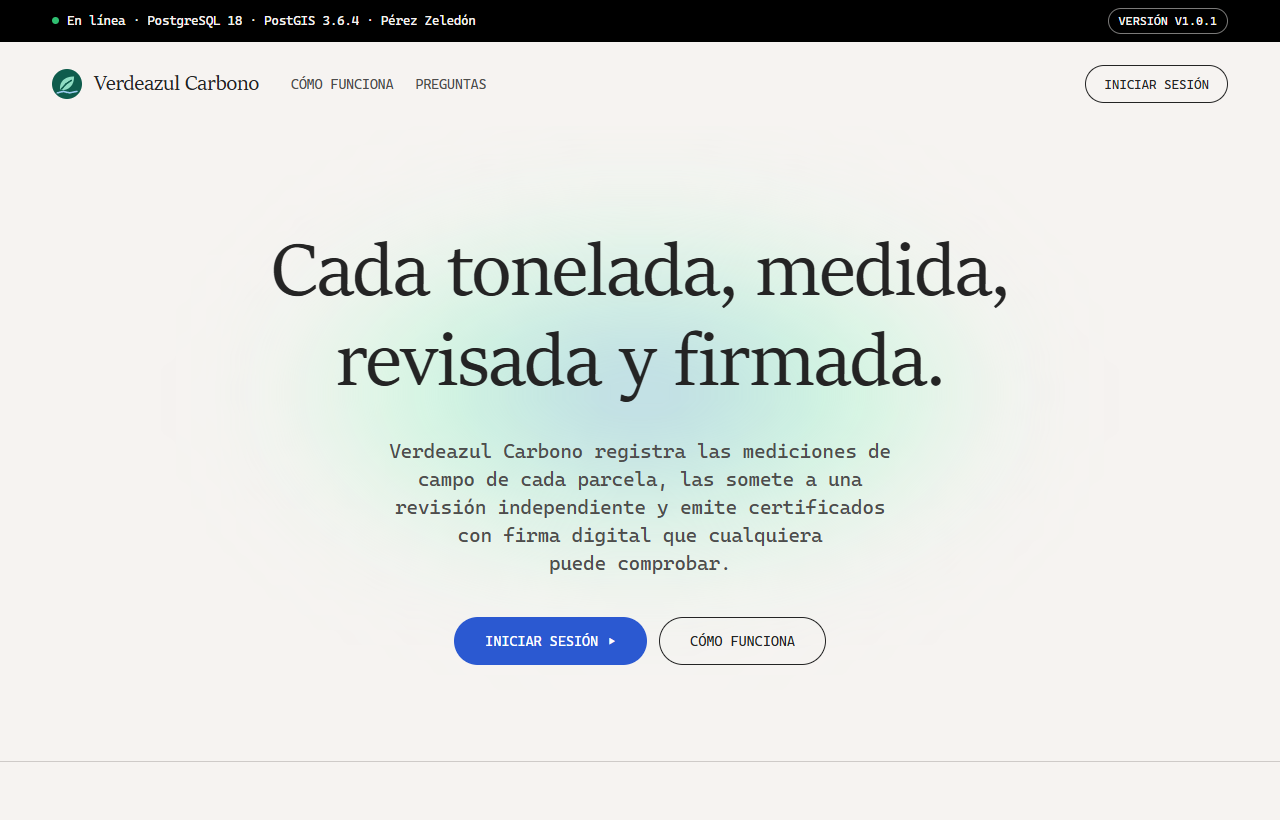
\includegraphics[width=0.42\textwidth]{../evidencia/01-app-https.png}
\caption{La portada de \cod{v1.0.0} en \url{https://verdeazul-app-708901712393.us-east1.run.app}. Las imágenes desplegadas y sus etiquetas, en el Anexo~B.}
\end{figure}

\subsection{Secret Manager}

\begin{salida}
\VerbatimInput{../evidencia/secret-manager.txt}
\end{salida}

\subsection{Dependabot activo}

\begin{figure}[H]
\centering
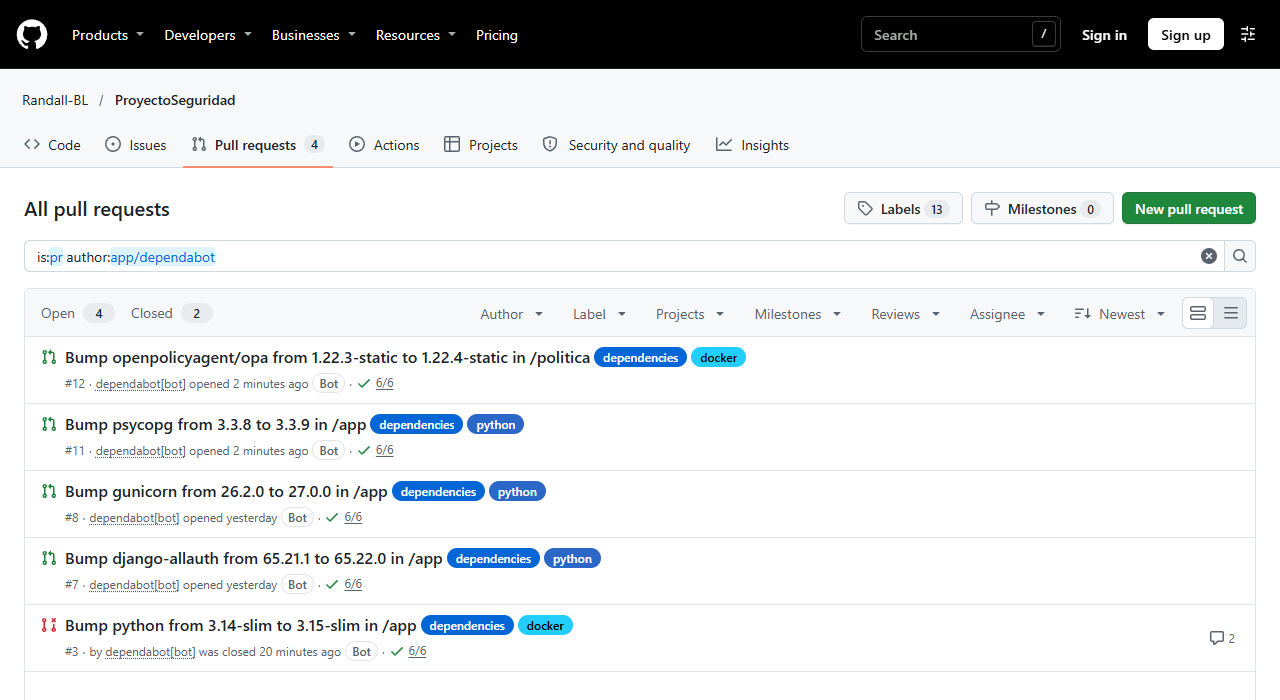
\includegraphics[width=0.55\textwidth]{../evidencia/05-dependabot-prs.png}
\caption{Las propuestas de Dependabot en el repositorio, el 15 de noviembre. El PR \#3 (Python 3.15)
se revisó y se cerró con la justificación escrita (tarea 9.2); las demás quedan para revisar con el
mismo procedimiento.}
\end{figure}

\subsection{Un certificado verificado y uno alterado}

\begin{figure}[H]
\centering
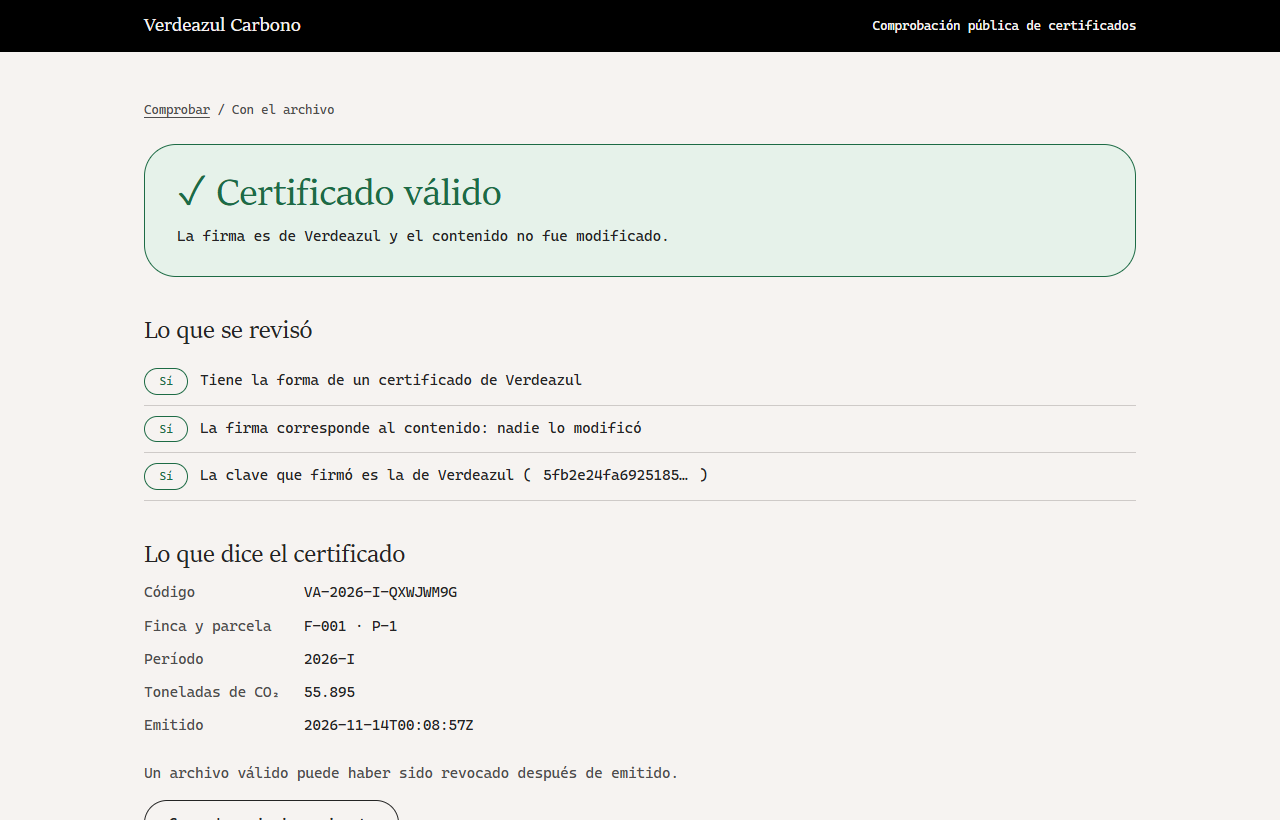
\includegraphics[width=0.49\textwidth]{../evidencia/02-certificado-valido.png}\hfill
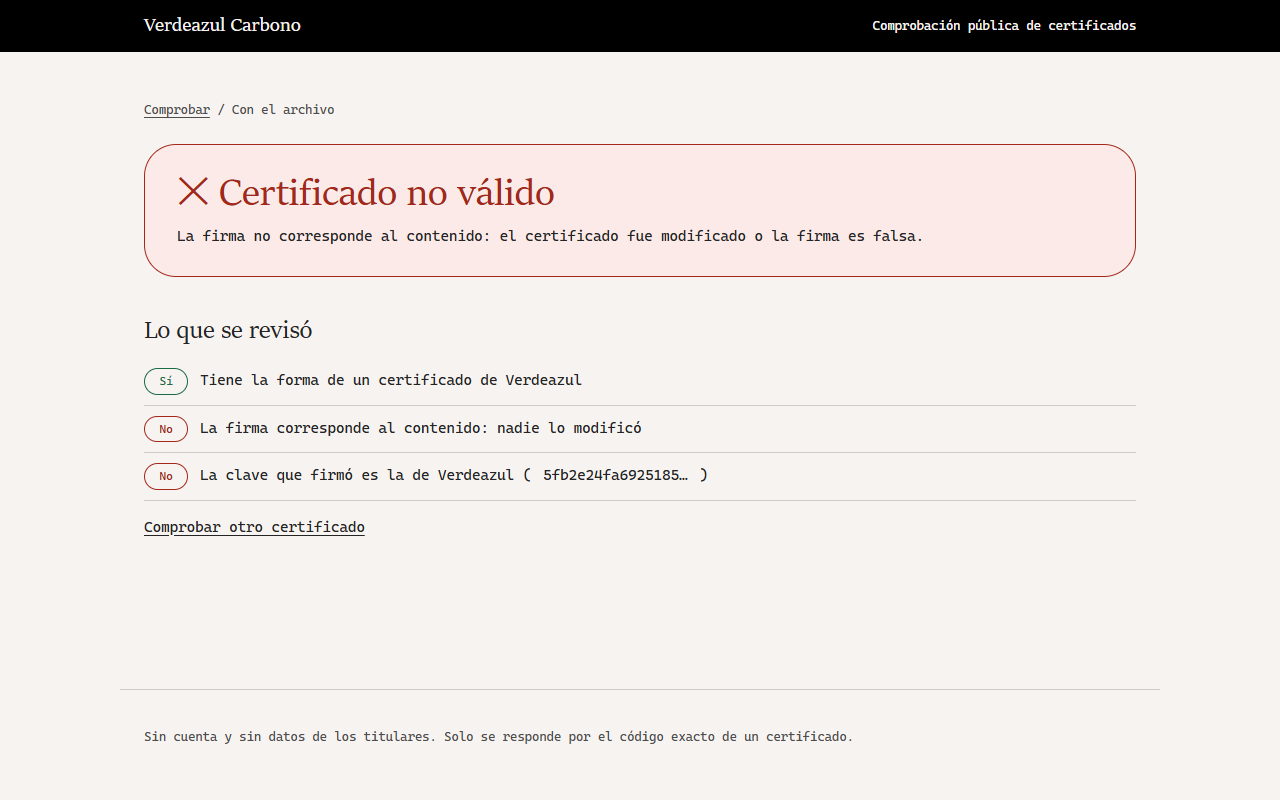
\includegraphics[width=0.49\textwidth]{../evidencia/03-certificado-alterado.png}
\caption{El servicio público con el certificado real \cod{VA-2026-I-QXWJWM9G} (izquierda) y con la
misma copia con una tonelada cambiada (derecha). Archivos en \cod{docs/demostracion/}; el verificador sin conexión da lo mismo (Anexo~B).}
\end{figure}

\subsection{El intento fallido de un rol}

\begin{figure}[H]
\centering
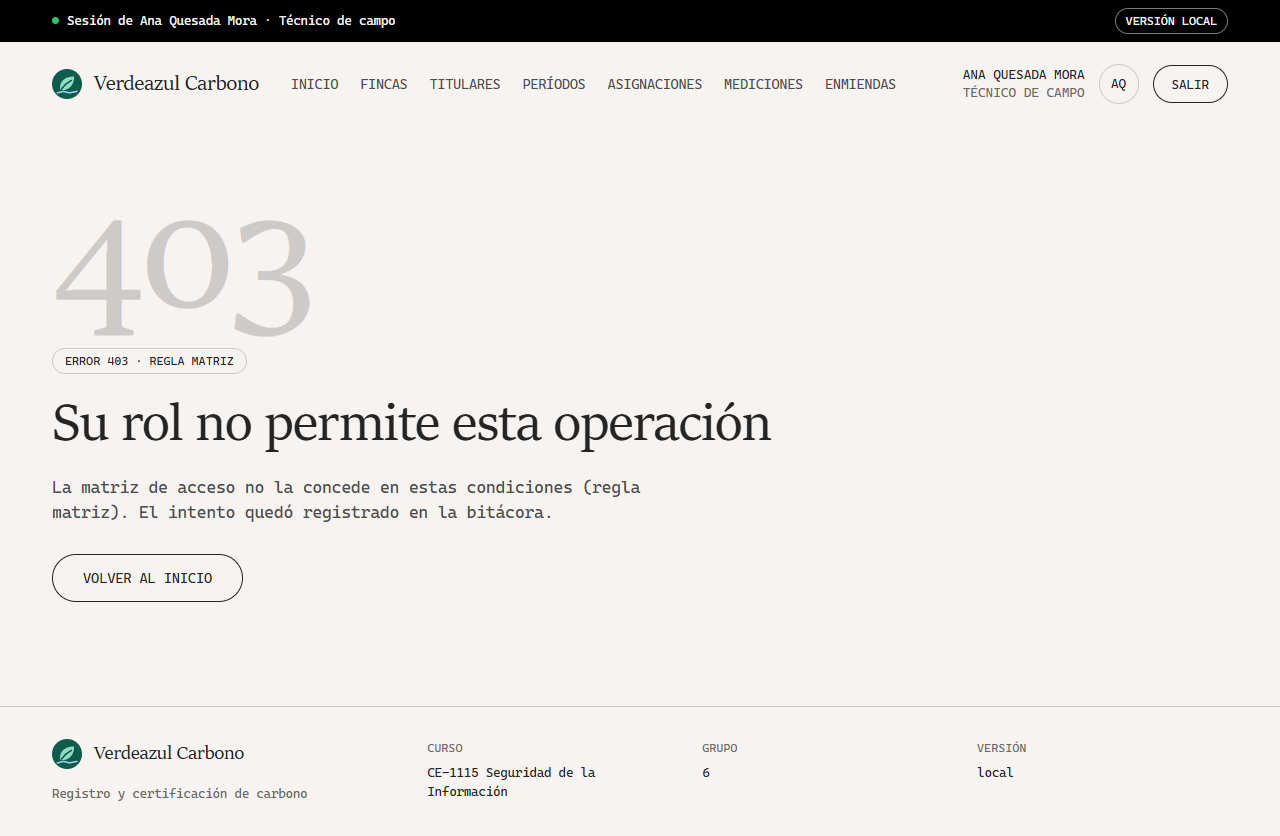
\includegraphics[width=0.49\textwidth]{../evidencia/06-tec-aprueba-sin-interfaz.png}\hfill
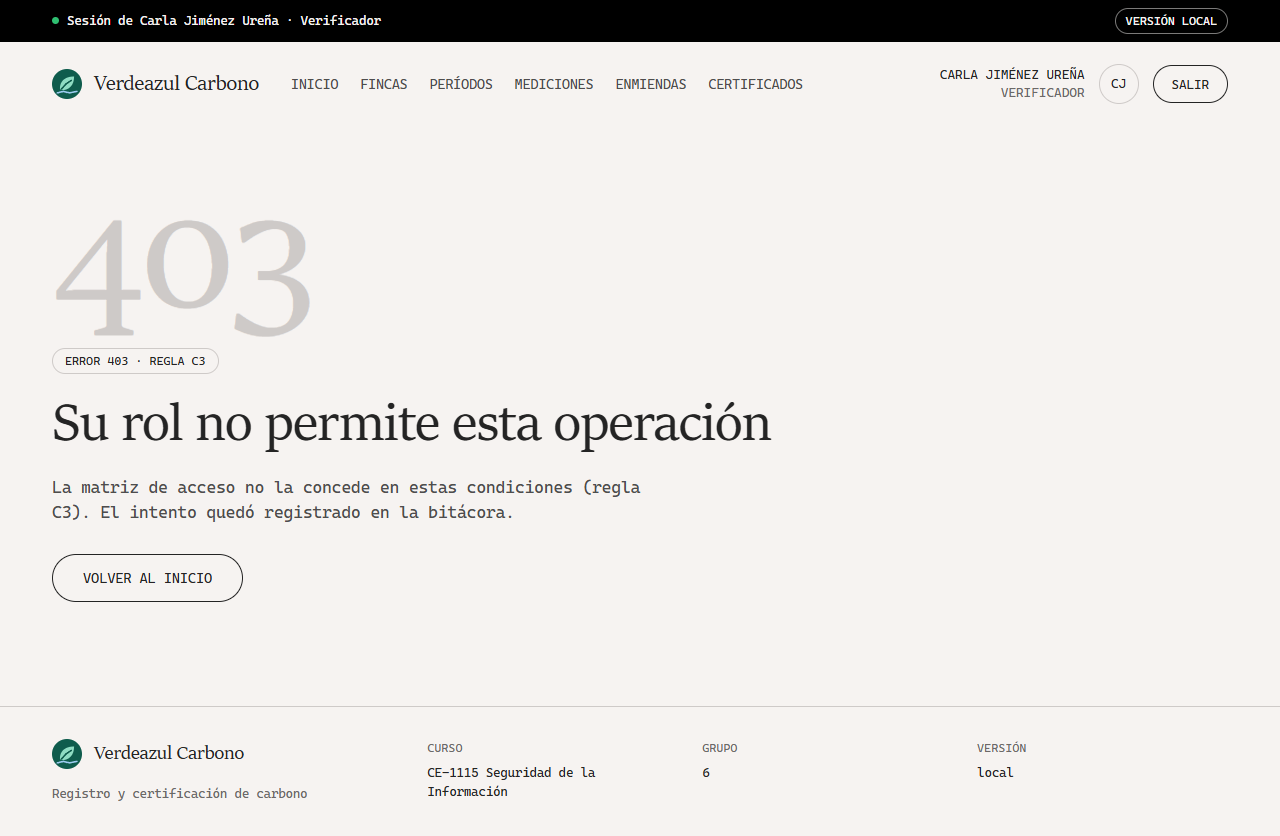
\includegraphics[width=0.49\textwidth]{../evidencia/07-ver-aprueba-lo-suyo-c3.png}
\caption{Izquierda: la técnica A envía a mano, con su sesión y su marca CSRF, la petición de aprobar
una medición; su rol no tiene ese verbo y el servidor la rechaza aunque la interfaz no muestre el
botón. Derecha: la verificadora C intenta aprobar una medición de la que escribió una versión: C3.}
\end{figure}

\begin{figure}[H]
\centering
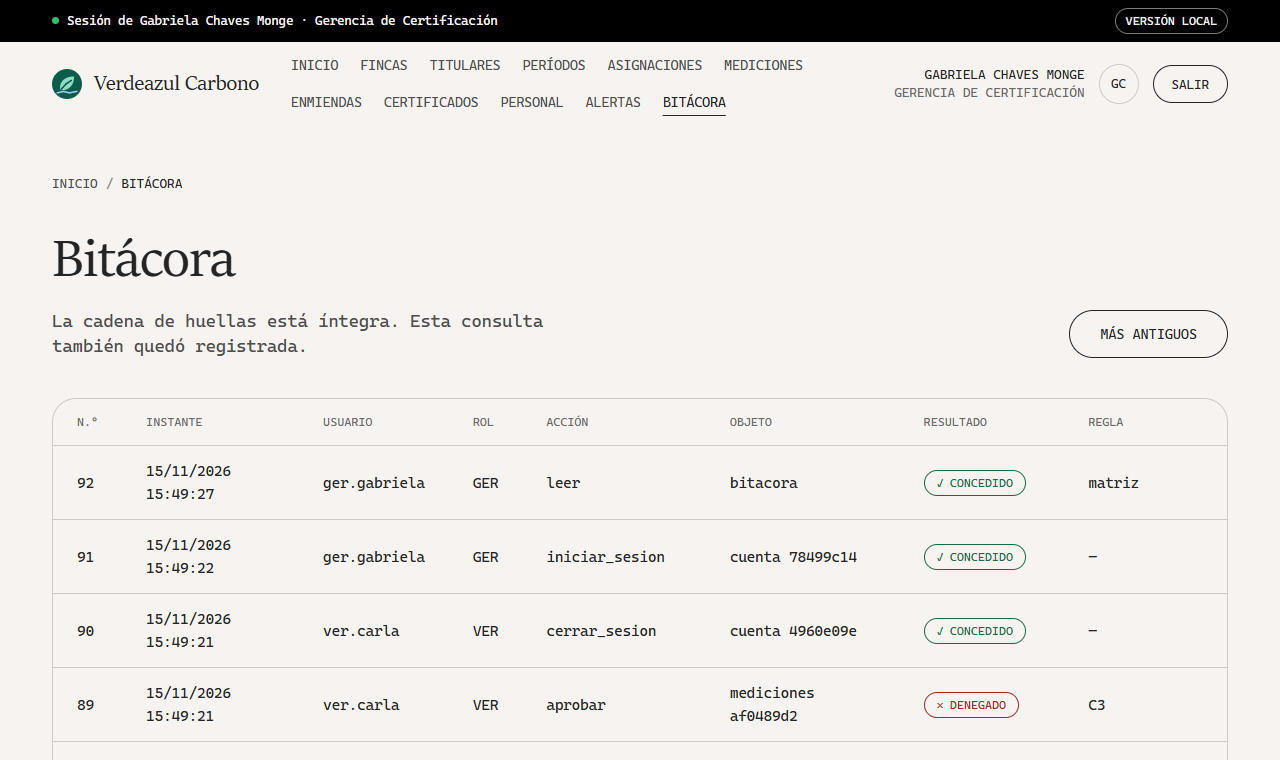
\includegraphics[width=0.5\textwidth]{../evidencia/08-bitacora-ger.png}
\caption{La bitácora vista por GER: los dos intentos quedaron como «denegado» con su regla (89: C3;
85: matriz), y la cadena de huellas está íntegra.}
\end{figure}


\newpage
\appendix
\section{Cobertura permiso por permiso}

Generada con \arch{infra/cobertura.py}. «Pantalla» quiere decir que la prueba entra con ese rol a la
ruta que lo ejerce; «objeto», que hay una prueba propia que hace la acción y comprueba el cambio. Todas
pasaron en las corridas del CI de \cod{v1.0.0} y de \cod{v1.0.1}.

\begin{center}
\scriptsize
\renewcommand{\arraystretch}{1.05}
\setlength{\tabcolsep}{3pt}
\begin{longtable}{@{}p{0.6cm} p{1.7cm} p{1.2cm} p{0.9cm} p{3.4cm} p{2.6cm} p{3.4cm} p{0.8cm}@{}}
\toprule
\cab{Rol} & \cab{Objeto} & \cab{Verbo} & \cab{Reglas} & \cab{Dónde (ruta o componente)} & \cab{Motor y base} & \cab{Prueba} & \cab{Resultado} \\
\midrule
\endhead
TEC & fincas & leer & C1 & fincas, \allowbreak{}finca & reglas.rego:17; negocio 0003, negocio 0005, negocio 0007 & (pantalla) & pasó \\
TEC & datos\_\allowbreak{}personales & leer & C1 & titulares, \allowbreak{}titular & reglas.rego:17; negocio 0003, negocio 0005, negocio 0007 & (pantalla) & pasó \\
TEC & periodos & leer & — & periodos, \allowbreak{}periodo & matriz.json & (pantalla) & pasó \\
TEC & asignaciones & leer & C1 & asignaciones & reglas.rego:17; negocio 0003, negocio 0005, negocio 0007 & (pantalla) & pasó \\
TEC & mediciones & leer & C1 & mediciones, \allowbreak{}medicion & reglas.rego:17; negocio 0003, negocio 0005, negocio 0007 & (pantalla) & pasó \\
TEC & mediciones & crear & C2 & nueva\_medicion & reglas.rego:34; negocio 0004 & test\_\allowbreak{}tec\_\allowbreak{}crear\_\allowbreak{}mediciones & pasó \\
TEC & mediciones & modificar & C2 & modificar\_medicion & reglas.rego:34; negocio 0004 & test\_\allowbreak{}tec\_\allowbreak{}modificar\_\allowbreak{}mediciones & pasó \\
TEC & mediciones & enviar & C2 & enviar\_medicion & reglas.rego:34; negocio 0004 & test\_\allowbreak{}tec\_\allowbreak{}enviar\_\allowbreak{}mediciones & pasó \\
TEC & enmiendas & leer & C1 & enmiendas, \allowbreak{}enmienda & reglas.rego:17; negocio 0003, negocio 0005, negocio 0007 & (pantalla) & pasó \\
TEC & enmiendas & solicitar & C7 & solicitar\_enmienda & reglas.rego:88 & test\_\allowbreak{}tec\_\allowbreak{}solicitar\_\allowbreak{}enmiendas & pasó \\
TEC & enmiendas & corregir & C9 & corregir\_enmienda & reglas.rego:105 & test\_\allowbreak{}tec\_\allowbreak{}corregir\_\allowbreak{}enmiendas & pasó \\
TEC & cuentas & modificar & C13 & mis\_vinculos & reglas.rego:145 & (pantalla) & pasó \\
VER & fincas & leer & H & fincas, \allowbreak{}finca & matriz.json & (pantalla) & pasó \\
VER & periodos & leer & — & periodos, \allowbreak{}periodo & matriz.json & (pantalla) & pasó \\
VER & mediciones & leer & H & mediciones, \allowbreak{}medicion & matriz.json & (pantalla) & pasó \\
VER & mediciones & aprobar & C3 & aprobar\_medicion & reglas.rego:51; negocio 0004 & test\_\allowbreak{}ver\_\allowbreak{}aprobar\_\allowbreak{}mediciones & pasó \\
VER & mediciones & devolver & C3 & devolver\_medicion & reglas.rego:51; negocio 0004 & test\_\allowbreak{}ver\_\allowbreak{}devolver\_\allowbreak{}mediciones & pasó \\
VER & enmiendas & leer & — & enmiendas, \allowbreak{}enmienda & matriz.json & (pantalla) & pasó \\
VER & enmiendas & solicitar & C7 & solicitar\_enmienda & reglas.rego:88 & test\_\allowbreak{}ver\_\allowbreak{}solicitar\_\allowbreak{}enmiendas & pasó \\
VER & enmiendas & revisar & C10 & revisar\_enmienda & reglas.rego:113; negocio 0004 & test\_\allowbreak{}ver\_\allowbreak{}revisar\_\allowbreak{}enmiendas & pasó \\
VER & certificados & leer & H & certificados, \allowbreak{}certificado, \allowbreak{}descargar\_certificado & matriz.json & (pantalla) & pasó \\
VER & cuentas & modificar & C13 & mis\_vinculos & reglas.rego:145 & (pantalla) & pasó \\
SUP & fincas & leer & H & fincas, \allowbreak{}finca & matriz.json & (pantalla) & pasó \\
SUP & periodos & leer & — & periodos, \allowbreak{}periodo & matriz.json & (pantalla) & pasó \\
SUP & asignaciones & leer & — & asignaciones & matriz.json & (pantalla) & pasó \\
SUP & asignaciones & crear & C19 & crear\_asignacion & reglas.rego:185; negocio 0004, negocio 0007 & (pantalla) & pasó \\
SUP & asignaciones & modificar & C19 & asignacion, \allowbreak{}terminar\_asignacion, \allowbreak{}renovar\_asignacion & reglas.rego:185; negocio 0004, negocio 0007 & test\_\allowbreak{}sup\_\allowbreak{}modificar\_\allowbreak{}asignaciones & pasó \\
SUP & mediciones & leer & H & mediciones, \allowbreak{}medicion & matriz.json & (pantalla) & pasó \\
SUP & enmiendas & leer & — & enmiendas, \allowbreak{}enmienda & matriz.json & (pantalla) & pasó \\
SUP & cuentas & modificar & C13 & mis\_vinculos & reglas.rego:145 & (pantalla) & pasó \\
SUP & alertas & leer & C15 & alertas & reglas.rego:164; negocio 0006 & (pantalla) & pasó \\
SUP & alertas & resolver & C15 & resolver\_alerta & reglas.rego:164; negocio 0006 & test\_\allowbreak{}sup\_\allowbreak{}resolver\_\allowbreak{}alertas & pasó \\
GER & fincas & leer & H & fincas, \allowbreak{}finca & matriz.json & (pantalla) & pasó \\
GER & fincas & aprobar & C11 & aprobar\_catalogo & reglas.rego:122; negocio 0004 & test\_\allowbreak{}ger\_\allowbreak{}aprobar\_\allowbreak{}fincas & pasó \\
GER & datos\_\allowbreak{}personales & leer & H & titulares, \allowbreak{}titular & matriz.json & (pantalla) & pasó \\
GER & periodos & leer & — & periodos, \allowbreak{}periodo & matriz.json & (pantalla) & pasó \\
GER & periodos & abrir & C14 & abrir\_periodo & reglas.rego:149; negocio 0004 & test\_\allowbreak{}ger\_\allowbreak{}abrir\_\allowbreak{}periodos & pasó \\
GER & periodos & cerrar & C14 & cerrar\_periodo & reglas.rego:149; negocio 0004 & test\_\allowbreak{}ger\_\allowbreak{}cerrar\_\allowbreak{}periodos & pasó \\
GER & asignaciones & leer & — & asignaciones & matriz.json & (pantalla) & pasó \\
GER & mediciones & leer & H & mediciones, \allowbreak{}medicion & matriz.json & (pantalla) & pasó \\
GER & enmiendas & leer & — & enmiendas, \allowbreak{}enmienda & matriz.json & (pantalla) & pasó \\
GER & enmiendas & solicitar & C7 & solicitar\_enmienda & reglas.rego:88 & test\_\allowbreak{}ger\_\allowbreak{}solicitar\_\allowbreak{}enmiendas & pasó \\
GER & enmiendas & autorizar & C8 & autorizar\_enmienda & reglas.rego:95; negocio 0004 & test\_\allowbreak{}ger\_\allowbreak{}autorizar\_\allowbreak{}enmiendas & pasó \\
GER & certificados & leer & H & certificados, \allowbreak{}certificado, \allowbreak{}descargar\_certificado & matriz.json & (pantalla) & pasó \\
GER & cuentas & leer & — & cuentas, \allowbreak{}cuenta & matriz.json & (pantalla) & pasó \\
GER & cuentas & aprobar & C12 & aprobar\_rol, \allowbreak{}aprobar\_retiro & reglas.rego:132; negocio 0004 & test\_\allowbreak{}ger\_\allowbreak{}aprobar\_\allowbreak{}cuentas & pasó \\
GER & cuentas & modificar & C13 & mis\_vinculos & reglas.rego:145 & (pantalla) & pasó \\
GER & bitacora & leer & — & bitacora & matriz.json & (pantalla) & pasó \\
GER & alertas & leer & — & alertas & matriz.json & (pantalla) & pasó \\
GER & alertas & resolver & C15 & resolver\_alerta & reglas.rego:164; negocio 0006 & test\_\allowbreak{}ger\_\allowbreak{}resolver\_\allowbreak{}alertas & pasó \\
ADM & fincas & leer & H & fincas, \allowbreak{}finca & matriz.json & (pantalla) & pasó \\
ADM & fincas & proponer & C11 & proponer\_finca, \allowbreak{}proponer\_titular, \allowbreak{}proponer\_parcela & reglas.rego:122; negocio 0004 & (pantalla) & pasó \\
ADM & datos\_\allowbreak{}personales & leer & H & titulares, \allowbreak{}titular & matriz.json & (pantalla) & pasó \\
ADM & datos\_\allowbreak{}personales & crear & — & crear\_titular & matriz.json & (pantalla) & pasó \\
ADM & datos\_\allowbreak{}personales & modificar & — & editar\_titular & matriz.json & test\_\allowbreak{}adm\_\allowbreak{}modificar\_\allowbreak{}datos\_\allowbreak{}personales & pasó \\
ADM & datos\_\allowbreak{}personales & eliminar & C16 & suprimir\_titular & reglas.rego:177; negocio 0004 & test\_\allowbreak{}adm\_\allowbreak{}eliminar\_\allowbreak{}datos\_\allowbreak{}personales & pasó \\
ADM & periodos & leer & — & periodos, \allowbreak{}periodo & matriz.json & (pantalla) & pasó \\
ADM & periodos & crear & — & crear\_periodo & matriz.json & (pantalla) & pasó \\
ADM & periodos & proponer & C14 & proponer\_periodo & reglas.rego:149; negocio 0004 & test\_\allowbreak{}adm\_\allowbreak{}proponer\_\allowbreak{}periodos & pasó \\
ADM & cuentas & leer & — & cuentas, \allowbreak{}cuenta & matriz.json & (pantalla) & pasó \\
ADM & cuentas & crear & C12 & crear\_cuenta & reglas.rego:132; negocio 0004 & (pantalla) & pasó \\
ADM & cuentas & desactivar & C12 & desactivar\_cuenta & reglas.rego:132; negocio 0004 & test\_\allowbreak{}adm\_\allowbreak{}desactivar\_\allowbreak{}cuentas & pasó \\
ADM & cuentas & proponer & C12 & proponer\_rol & reglas.rego:132; negocio 0004 & test\_\allowbreak{}adm\_\allowbreak{}proponer\_\allowbreak{}cuentas & pasó \\
ADM & cuentas & modificar & C13 & mis\_vinculos & reglas.rego:145 & (pantalla) & pasó \\
AUD & fincas & leer & C6 & fincas, \allowbreak{}finca & reglas.rego:84 & (pantalla) & pasó \\
AUD & fincas & exportar & C18 & exportar\_fincas & reglas.rego:180 & (pantalla) & pasó \\
AUD & datos\_\allowbreak{}personales & leer & C6 & titulares, \allowbreak{}titular & reglas.rego:84 & (pantalla) & pasó \\
AUD & periodos & leer & C6 & periodos, \allowbreak{}periodo & reglas.rego:84 & (pantalla) & pasó \\
AUD & periodos & exportar & C18 & exportar\_periodos & reglas.rego:180 & (pantalla) & pasó \\
AUD & asignaciones & leer & C6 & asignaciones & reglas.rego:84 & (pantalla) & pasó \\
AUD & asignaciones & exportar & C18 & exportar\_asignaciones & reglas.rego:180 & (pantalla) & pasó \\
AUD & mediciones & leer & C6 & mediciones, \allowbreak{}medicion & reglas.rego:84 & (pantalla) & pasó \\
AUD & mediciones & exportar & C18 & exportar\_mediciones & reglas.rego:180 & (pantalla) & pasó \\
AUD & enmiendas & leer & C6 & enmiendas, \allowbreak{}enmienda & reglas.rego:84 & (pantalla) & pasó \\
AUD & enmiendas & exportar & C18 & exportar\_enmiendas & reglas.rego:180 & (pantalla) & pasó \\
AUD & certificados & leer & C6 & certificados, \allowbreak{}certificado, \allowbreak{}descargar\_certificado & reglas.rego:84 & (pantalla) & pasó \\
AUD & certificados & exportar & C18 & exportar\_certificados & reglas.rego:180 & (pantalla) & pasó \\
AUD & cuentas & leer & C6 & cuentas, \allowbreak{}cuenta & reglas.rego:84 & (pantalla) & pasó \\
AUD & cuentas & modificar & C13 & mis\_vinculos & reglas.rego:145 & (pantalla) & pasó \\
AUD & bitacora & leer & C6 & bitacora & reglas.rego:84 & (pantalla) & pasó \\
AUD & bitacora & exportar & C18 & exportar\_bitacora & reglas.rego:180 & (pantalla) & pasó \\
AUD & alertas & leer & C6 & alertas & reglas.rego:84 & (pantalla) & pasó \\
AUD & alertas & exportar & C18 & exportar\_alertas & reglas.rego:180 & (pantalla) & pasó \\
DUE & fincas & leer & C5 & fincas, \allowbreak{}finca & reglas.rego:72; negocio 0003, negocio 0007 & (pantalla) & pasó \\
DUE & datos\_\allowbreak{}personales & leer & C5 & titulares, \allowbreak{}titular & reglas.rego:72; negocio 0003, negocio 0007 & (pantalla) & pasó \\
DUE & periodos & leer & — & periodos, \allowbreak{}periodo & matriz.json & (pantalla) & pasó \\
DUE & asignaciones & leer & C5 & asignaciones & reglas.rego:72; negocio 0003, negocio 0007 & (pantalla) & pasó \\
DUE & mediciones & leer & C5 & mediciones, \allowbreak{}medicion & reglas.rego:72; negocio 0003, negocio 0007 & (pantalla) & pasó \\
DUE & enmiendas & leer & C5 & enmiendas, \allowbreak{}enmienda & reglas.rego:72; negocio 0003, negocio 0007 & (pantalla) & pasó \\
DUE & certificados & leer & C5 & certificados, \allowbreak{}certificado, \allowbreak{}descargar\_certificado & reglas.rego:72; negocio 0003, negocio 0007 & (pantalla) & pasó \\
DUE & cuentas & modificar & C13 & mis\_vinculos & reglas.rego:145 & (pantalla) & pasó \\
SIS & fincas & leer & — & emision/emitir.py (lee lo necesario para emitir con va\_emision) & matriz.json & test\_\allowbreak{}emite\_\allowbreak{}una\_\allowbreak{}medicion\_\allowbreak{}aprobada\_\allowbreak{}con\_\allowbreak{}contenido\_\allowbreak{}firmado & pasó \\
SIS & datos\_\allowbreak{}personales & leer & — & emision/emitir.py (lee lo necesario para emitir con va\_emision) & matriz.json & test\_\allowbreak{}emite\_\allowbreak{}una\_\allowbreak{}medicion\_\allowbreak{}aprobada\_\allowbreak{}con\_\allowbreak{}contenido\_\allowbreak{}firmado & pasó \\
SIS & periodos & leer & — & emision/emitir.py (lee lo necesario para emitir con va\_emision) & matriz.json & test\_\allowbreak{}emite\_\allowbreak{}una\_\allowbreak{}medicion\_\allowbreak{}aprobada\_\allowbreak{}con\_\allowbreak{}contenido\_\allowbreak{}firmado & pasó \\
SIS & asignaciones & leer & — & emision/emitir.py (lee lo necesario para emitir con va\_emision) & matriz.json & test\_\allowbreak{}emite\_\allowbreak{}una\_\allowbreak{}medicion\_\allowbreak{}aprobada\_\allowbreak{}con\_\allowbreak{}contenido\_\allowbreak{}firmado & pasó \\
SIS & mediciones & leer & — & emision/emitir.py (lee lo necesario para emitir con va\_emision) & matriz.json & test\_\allowbreak{}emite\_\allowbreak{}una\_\allowbreak{}medicion\_\allowbreak{}aprobada\_\allowbreak{}con\_\allowbreak{}contenido\_\allowbreak{}firmado & pasó \\
SIS & enmiendas & leer & — & emision/emitir.py (lee lo necesario para emitir con va\_emision) & matriz.json & test\_\allowbreak{}emite\_\allowbreak{}una\_\allowbreak{}medicion\_\allowbreak{}aprobada\_\allowbreak{}con\_\allowbreak{}contenido\_\allowbreak{}firmado & pasó \\
SIS & certificados & emitir & C4 & emision/emitir.py: emitir() (6.3) & reglas.rego:58; negocio 0002, negocio 0006 & test\_\allowbreak{}emite\_\allowbreak{}una\_\allowbreak{}medicion\_\allowbreak{}aprobada\_\allowbreak{}con\_\allowbreak{}contenido\_\allowbreak{}firmado & pasó \\
SIS & certificados & revocar & C4 & emision/emitir.py: reemitir() (6.5) & reglas.rego:58; negocio 0002, negocio 0006 & test\_\allowbreak{}t25\_\allowbreak{}una\_\allowbreak{}enmienda\_\allowbreak{}que\_\allowbreak{}cambia\_\allowbreak{}toneladas\_\allowbreak{}revoca\_\allowbreak{}y\_\allowbreak{}reemite & pasó \\
SIS & bitacora & anexar & — & bitacora\_anexar() en cada acción & matriz.json & test\_\allowbreak{}la\_\allowbreak{}cadena\_\allowbreak{}de\_\allowbreak{}la\_\allowbreak{}semilla\_\allowbreak{}esta\_\allowbreak{}integra & pasó \\
SIS & alertas & crear & — & autorizacion/historial.py: alertar() (alertas de H1 a H3) & matriz.json & test\_\allowbreak{}t18\_\allowbreak{}h1\_\allowbreak{}mas\_\allowbreak{}fincas\_\allowbreak{}que\_\allowbreak{}el\_\allowbreak{}umbral\_\allowbreak{}pide\_\allowbreak{}segundo\_\allowbreak{}factor\_\allowbreak{}y\_\allowbreak{}motivo & pasó \\
PUB & certificados & comprobar & C20 & publico/servicio.py: /comprobar (6.7) & reglas.rego:193; negocio 0006 & test\_\allowbreak{}un\_\allowbreak{}codigo\_\allowbreak{}vigente & pasó \\
\bottomrule
\end{longtable}
\end{center}


\section{Salidas completas}

\subsection*{Lo que corre en Cloud Run y en Artifact Registry}
\begin{salida}
\VerbatimInput{../evidencia/cloud-run.txt}
\end{salida}

\subsection*{El verificador sin conexión}
\begin{salida}
\VerbatimInput{../evidencia/verificador.txt}
\end{salida}

\end{document}
